% This must be in the first 5 lines to tell arXiv to use pdfLaTeX, which is strongly recommended.
\pdfoutput=1
% In particular, the hyperref package requires pdfLaTeX in order to break URLs across lines.

\documentclass[11pt]{article}

% Remove the "review" option to generate the final version.
\usepackage{ACL2023}

% Standard package includes
\usepackage{times}
\usepackage{latexsym}

% For proper rendering and hyphenation of words containing Latin characters (including in bib files)
\usepackage[T1]{fontenc}
% For Vietnamese characters
% \usepackage[T5]{fontenc}
% See https://www.latex-project.org/help/documentation/encguide.pdf for other character sets

% This assumes your files are encoded as UTF8
\usepackage[utf8]{inputenc}

% This is not strictly necessary, and may be commented out.
% However, it will improve the layout of the manuscript,
% and will typically save some space.
\usepackage{microtype}

% This is also not strictly necessary, and may be commented out.
% However, it will improve the aesthetics of text in
% the typewriter font.
\usepackage{inconsolata}


% If the title and author information does not fit in the area allocated, uncomment the following
%
%\setlength\titlebox{<dim>}
%
% and set <dim> to something 5cm or larger.

\title{Info 555 Project 1: Diachronic Linguistic Analysis of Topic-Specific Corpus}

% Author information can be set in various styles:
% For several authors from the same institution:
% \author{Author 1 \and ... \and Author n \\
%         Address line \\ ... \\ Address line}
% if the names do not fit well on one line use
%         Author 1 \\ {\bf Author 2} \\ ... \\ {\bf Author n} \\
% For authors from different institutions:
% \author{Author 1 \\ Address line \\  ... \\ Address line
%         \And  ... \And
%         Author n \\ Address line \\ ... \\ Address line}
% To start a seperate ``row'' of authors use \AND, as in
% \author{Author 1 \\ Address line \\  ... \\ Address line
%         \AND
%         Author 2 \\ Address line \\ ... \\ Address line \And
%         Author 3 \\ Address line \\ ... \\ Address line}

\author{Joshua Dunlap \\
 joshdunlapc@arizona.edu \\\An
   \\
 \\
   \\
   \\
  \texttt\\}

\begin{document}
\maketitle


\section{Project}

My project is to create word embeddings for a specific, time-stamped corpus—the entirety of the online hosted (\href{https://theanarchistlibrary.org/}{https://theanarchistlibrary.org}) Anarchist Library—in order to analyze semantic shifts in the corpus over time. The foundational idea is that of diachronic linguistics which “concerns itself with the process of language development over time and, in particular, with questions [of] why and how languages change and in which way these changes spread across [the] spatio-temporal dimension” (Jatowt and Duh, 2014). While I encountered past scholarship (referenced below in the “related work” section) that sought to measure general language shift, my project seeks to see how language use changes over time in a topic-specific corpus in which many of the authors understand themselves to be in conversation with each other or engaging with some of the same historical reference points. My general hypothesis is that because one cause of language change is cultural shift (Hamilton et al., 2016a) a topic-specific corpus will be able to register these changes at a granular level particular to the community of authors and readers. In this case: cultural shifts internal to anarchist/revolutionary politics will be discernible by diachronic linguistic analysis on this corpus while they would not be discernible using a model trained on a broader corpus.


\section{Method}

This project, then, consists of two major components. The first is transforming the 30,000 documents on The Anarchist Library into a usable dataset, while the second is training a Word2Vec model on those data and performing analyses on the temporal changes in language use to be found in the model.

To start, the entirety of The Anarchist Library website was downloaded to local disk using the website’s robots.txt (\href{https://theanarchistlibrary.org/robots.txt}{https://theanarchistlibrary.org/robots.txt}). The resulting folder had a size of about 12GB and what appeared to be a lot of redundancy (file.a4.pdf, file.epub, file.html, etc.). From this folder, files ending in “.html” were extracted, converted to .txt, added to a single corpus, and written as a .json file—the final product with a size of about 1.5GB. 

Next, I went through a series of text pre-processing steps to prepare the documents to be used to build the Word2Vec model: tokenization, (some degree of) text normalization, stop word removal, decade extraction. Here, I noticed an issue with my plan to measure semantic change over time. I had intended to create a Word2Vec model for each decade in the corpus and then measure change over time by measuring cosine similarity between a given term in some decade and the same term in subsequent decades. I realized, however, that because Word2Vec models are randomly initialized, cosine similarity between different models would be a meaningless measure. While semantic relationships internal to a model are maintained, the direction of a given concept would change from model to model (see “limitations/future projects” section below for more discussion). With this in mind, I elected to append the decade of the document a given word appears in to each word in the corpus in order to be able to generate a single Word2Vec model for the entire corpus. I elected to make a skipgram model with a window of 5 in large part because of the supporting literature I read (see “related work” section), and after some adjustments I landed on a minimum count of 5 for a word for inclusion, largely as an effort to exclude rare/irrelevant words from nearest neighbor lists later on. Computational limitations prevented me from tuning the parameters of the model as much as I would have liked—this is documented in more detail below.



\section{Related Work}

I was inspired in this project by the existing literature on diachronic computational linguistics, especially work considering sociolinguistic explanations for semantic change over time (Jatowt and Duh, 2014). Several of the works I read in preparation for—and as I was working on—this project noted that broader cultural shifts can be registered by a change in nearest neighbors to a word embeddings, with the paradigmatic example being the historically recent shift in nearest neighbors for the word “gay” from words like “frolicsome” and “young” to words like “lesbian” and “community” (ibid) (Hamilton et al, 2016a). From these earlier works, I took inspiration to measure time in decade intervals, to use a skipgram model, and to analyze “semantic change of single word[s]” using a “local neighborhood measure.” I feel my project takes on a type of work that I found few examples of, that of analyzing cultural shifts of a specific community by working on a community-specific corpus. The closest I found to this was scholarship on the emergence of Dutch nationalism by analyzing Dutch literature over a period of 200 years (Timmermans et al, 2022). Notably however, Timmermans et al. are still analyzing at the level of a national community, not at a smaller and more topically focused level.


\section{Experiments}


My experiments, like those of the papers I cited in the related work section, were a series of case studies on single words or word pairs to measure semantic shift over time. First, I wrote functions to: 1. Count, in decade intervals, from a given decade up to the present. 2. Given a term and start decade, display the term’s 5 nearest neighbors (in cosine similarity) from the start decade to present, and 3. Track, for the purpose of direct comparisons, the cosine similarity of two provided terms from a start decade to present. I also wrote code to plot the similarity over time provided by this last function. 

For case studies, I attempted to identify words/word pairs that would drive at various types of cultural semantic shift: technological, historical, developments in theory/practice, as well as a control (specific to the corpus) that indicates the relative stability of certain language use over time. These concepts roughly pair with types of cultural shift measured in the supporting literature; as in the oft cited shift of meaning of “mouse” from similar to “rat” to similar to “click” and “point” as an example of technologically driven cultural change of language (Jatowt and Duh, 2014).


\section{
Analyses/Results
}
Case Studies:

\subsection{Control
}



First, I looked at the term “marx” (all terms lowercase) in the corpus from the 1970s to the 2020s, finding that the term has notable stability across this time period. In these six decades, the most similar term is “engels” five out of six times, and “engels” is in the top five nearest neighbors in the one decade (1980s) that it is not the closest term. Additionally, there is a lot of stability in terms of the other close terms and the other \textit{type} of close terms. Several times we also see “karl”, and we also tend to see other 19th century revolutionary communist/anarchist philosophers, “proudhon”, “bakunin”, and “kropotkin.” Charting the similarity between “marx” and “engels” over time we see high and stable similarity across this time period (see Figure 1). Setting the starting decade earlier introduces more noise to the nearest neighbors (words like “perhaps” and “released”) though it does not significantly impact cosine similarity over time with “engels”—an issue I’ll address in the next case study.


\subsection{Historical}

Next, I sought to understand cultural shifts in language use related to historical events, one recent and one more distant. For the recent historical event, I analyzed the word “occupy” alongside words related to the Occupy Wall Street (OWS) movement. First a note on tracking similarities of two words across time. This case study allowed me to realize a problem with the dataset: tracking the similarity between “occupy” and “park” (many occupy protests were held in public parks) from 1900 to 2020 shows a major \textit{dip} in similarity as the analysis gets closer to the present (see Figure 2). After corroborating this trend with several other word pairs, I determined that the lopsided nature of the data—several times more documents in recent decades as opposed to decades further in the past—boosted the cosine similarity for decades with lower document counts. After this realization, I stopped using word pairs over time (see “limitations/future projects”). Nevertheless, the nearest neighbors are still instructive as they measure closest words \textit{internal to the same decade} and thus can reveal cultural shifts as the sort of words one finds as nearest neighbors change over time. In the case of “occupy”: earlier decades return words like “colonial”, “indians”, and “destiny” showing a relationship between “occupy” and the concept of colonization, as well as “shops”, “collectivise”, “secretaries”, and “corridors” suggesting workplace occupations or takeovers. Beginning in the 2010s and continuing into the 2020s we see “ows” (the movement itself), “zucotti” (the park where it began), “m15” (a related movement in Spain), “encampments” (the form of the protest), “squares” (held in plazas, squares, parks, also related/contemporaneous “movement of the squares” in Europe), etc. 

Looking to a more distant historical event, I analyzed the word “spanish” over time to relatively surprising results (see Image 1). More recent decades (1990s-2020s) reference the Spanish Civil War (a historically important event for the corpus in which anarchists pursued a revolution alongside their fight to prevent the fascist takeover of Spain by Francisco Franco) with terms like “1936-39” (the years of the war), “revolution/civil”, and “anarchosyndicalists.” More distant decades’ neighbors, in contrast, are largely just other nationalities: “japanese”, “italian”, “polish”, etc. This holds true for decades immediately preceding \textit{and }following the civil war itself, with the exception of the 1930s—the decade of the war—where we see “civil” and “fai” (acronym for a key anarchist organization in the war). This suggests that, outside of the writing that was being published as the war was taking place, perhaps it rose to historical significance in this corpus decades later, in the 1990s, alongside some sort of renewed interest in, or study of, the conflict.

\subsection{Technological}

I aimed also to capture cultural shifts related to changing technology that would be particular to this corpus. To illustrate one such change, we can look at the changing use of the word “signal” over time. While I imagine that in a broader corpus one may also see changes in this word, it holds a special meaning in this corpus as “signal” is the name of an encrypted messaging app that was launched in 2013 and is now in wide use by activists/those interested in revolutionary politics. We see from the beginning to the middle of the 20th century that there appears to be some religious association with the word, with neighbors like “preacher”, “demon”, and “prophetic”, while in the 2010s and 2020s we see rather direct associations with the app with words like “metadata”, “geolocation”, “relay”, and “accounts.”

\subsection{Theory/Practice}

Finally, I sought to capture changes to the theory and practice described in the corpus. With the word “disobedience” as a case study, we can see how the term shifts over time from what seems to be a question of individual defiance to a set of practices informed by theories of social movement tactics and strategy. In the late 1800s through the first half of the 1900s, closest neighbors are words like “pride”, “childlike”, “severest”, and “crude.” By the 1990s and extending into the present “non-violent” is in the top five every time, and it is accompanied by words like “gandhi’s” and “sit-downs”, as well as the sorts of campaigns that would likely employ civil disobedience, “anti-fracking” and “act-up’s” (referring to the grassroots AIDS activism group). With this example we can see how some words come to be used in a specialized theoretical manner and, consequently, their nearest neighbors change to reflect this. 

\section*{Limitations/Future Projects}
What follows are brief descriptions of limitations of the current project with directions for future work to improve the model/strengthen the findings.

As noted above, the decades are not aligned in vector space, so I cannot make direct comparisons of a term with itself over time. One of the works I was inspired by created a method to do this (it can be viewed here: \href{https://github.com/williamleif/histwords/blob/master/vecanalysis/alignment.py}{https://github.com/williamleif/histwords/blob/master/vecanalysis/alignment.py}), but I elected to not try to implement it on my project because I wanted to create my work from scratch rather than try to implement someone else’s solution (Hamilton et al, 2016b). It could be interesting to try to use their alignment tool in the future on this corpus.

Compute issues limited the scope of the project somewhat. Attempts to even tokenize the whole dataset on my laptop caused it to crash, while trying to build the model on Google Colab caused the runtime to restart due to running out of RAM. Eventually I built the model on a desktop, though it took about 40 minutes to run, so I was only able to change it a couple times. Future versions of this project could implement batching/use GPUs in order to avoid these issues.

As I described in the “analysis/results” section, I eventually stopped using the cosine similarity over time between two terms because smaller corpus size in earlier decades was distorting the outcomes—in smaller corpora in the earlier decades, most terms have a cosine similarity in the high 90s. Though it seems to me that meaningful results could still be drawn using the nearest neighbors method, inevitably some noise enters the data with less robust corpora. I’m curious if there’s weighting that could alleviate some of these issues, or whether there’s a minimum corpus size and some of the decades simply cannot be used. 

In the future I would like to compare some of the semantic shifts observed in this dataset to a large model pre-trained on more general data. This seems like it would be worthwhile because I could, potentially, show the comparative stability of a given term in a general time-stamped corpus alongside the changes to the term in the more specific corpus. With the examples above, I trust it is evident that, for example, in a more general corpus the term “spanish” does not come increasingly to talk about the Spanish Civil War, it would still likely be fruitful to make some of these comparisons between the specialized and the general change over time.


\section*{References}
William L. Hamilton, Jure Leskovec, and Dan Jurafsky. 2016.\href{https://aclanthology.org/D16-1229}{ Cultural Shift or Linguistic Drift? Comparing Two Computational Measures of Semantic Change}. In \textit{Proceedings of the 2016 Conference on Empirical Methods in Natural Language Processing}, pages 2116–2121, Austin, Texas. Association for Computational Linguistics.

William L. Hamilton, Jure Leskovec, and Dan Jurafsky. 2016.\href{https://aclanthology.org/P16-1141}{ Diachronic Word Embeddings Reveal Statistical Laws of Semantic Change}. In \textit{Proceedings of the 54th Annual Meeting of the Association for Computational Linguistics (Volume 1: Long Papers)}, pages 1489–1501, Berlin, Germany. Association for Computational Linguistics.

Adam Jatowt and Kevin Duh. 2014. A framework for analyzing semantic change of words across time. In \textit{Proceedings of the IEEE/ACM Joint Conference on Digital Libraries}, pages 229–238, London, UK. IEEE. https://doi.org/10.1109/JCDL.2014.6970173.

Marije Timmermans, Eva Vanmassenhove, and Dimitar Shterionov. 2022.\href{https://aclanthology.org/2022.lchange-1.13}{ “Vaderland”, “Volk” and “Natie”: Semantic Change Related to Nationalism in Dutch Literature Between 1700 and 1880 Captured with Dynamic Bernoulli Word Embeddings}. In \textit{Proceedings of the 3rd Workshop on Computational Approaches to Historical Language Change}, pages 125–130, Dublin, Ireland. Association for Computational Linguistics.


\section*{Figures/Images}
\begin{figure}
    \centering
    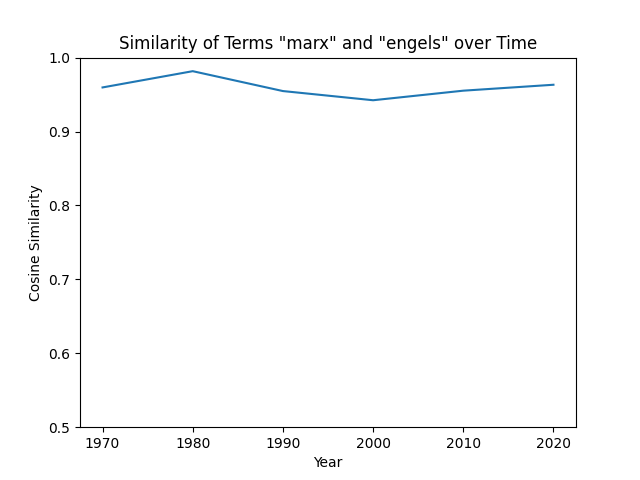
\includegraphics[width=0.5\linewidth]{marx-engels.png}
    \caption{Enter Caption}
    \label{Figure 1}
\end{figure}
\begin{figure}
    \centering
    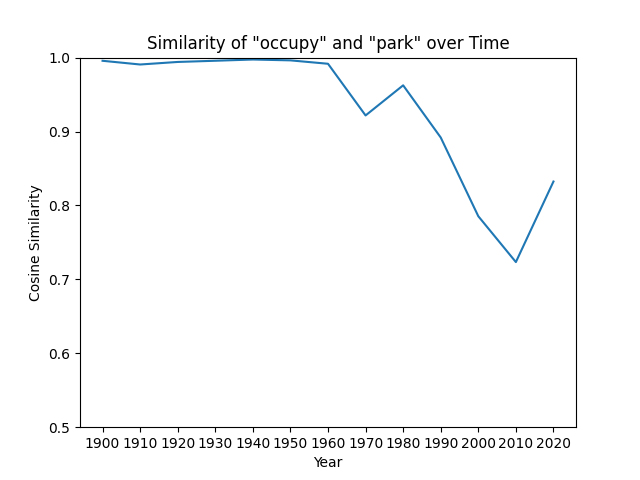
\includegraphics[width=0.5\linewidth]{occupy-park.png}
    \caption{Enter Caption}
    \label{fig:enter-label}
\end{figure}
\begin{figure}
    \centering
    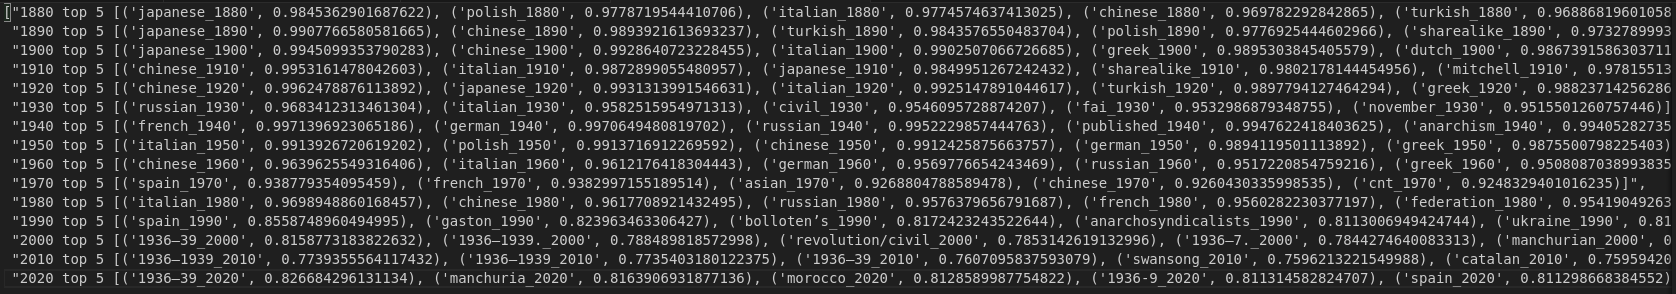
\includegraphics[width=0.5\linewidth]{spanish.png}
    \caption{Enter Caption}
    \label{fig:enter-label}
\end{figure}



\end{document}
